\chapter{Comportamento del sistema}
Rappresenta una \textbf{vista dinamica} del sistema, in cui si descrive il comportamento
degli agenti in termini della sequenza temporale di stati e le variabili che essi 
controllano.

Sostanzialmente vogliamo rappresentare come il sistema, sotto il controllo degli agenti 
verrà guidato in due possibili modalità:
\begin{itemize}
    \item Mediante una singola istanza di esecuzione
    \item Mediante classi di esecuzione
\end{itemize}
Entrambe le viste possono rappresentare il \textit{system as-is} o il \textit{system to-be}.

Tali viste possono avere molteplici utilizzi, infatti gli scenari possono essere
utilizzati in fase di elicitazione dei requisiti, per definire i casi d'uso, per
definire i test di sistema e per definire i test di accettazione.
Gli scenari sono un veicolo per la fase di elicitazione dei requisiti, in quanto
infatti possono far emergere domande sul perché determinate 
azioni devono essere intraprese.

Le state machine possono essere usate per supportare strumenti avanzati come le 
animazioni, model checking e generazione di codice.
\section{Modellare singole istanze di comportamenti}
\begin{tcolorbox}[colback=lime!5!white,colframe=lime!75!black, title=Scenario]
    Lo scenario rappresenta una successione temporale di eventi tra le varie istanze di 
    agenti che abbiamo disponibili nel nostro sistema.
\end{tcolorbox}
È possibile considerare tali sequenze fra differenti agenti, o diverse istanze di 
agenti dello stesso tipo.

Le interazioni possono avere diverse direzioni:
\begin{itemize}
    \item \textbf{Da} un'istanza di agente, che controlla l'evento.
    \item \textbf{Verso} un'istanza di agente, che monitora l'evento.
\end{itemize}
Gli scenari si contraddistinguono in:
\begin{itemize}
    \item \textbf{Scenari positivi}: rappresentano il raggiungimento di un goal 
    all'interno del sistema. Se di dividono a loro volta in:
    \begin{itemize}
        \item \textbf{Scenari normali}: rappresentano il raggiungimento di un goal
        senza particolari ostacoli.
        \item \textbf{Scenari anomali}: rappresentano il raggiungimento di un goal 
        nel caso in cui si verifichino particolari ostacoli (\textit{rimedio all'ostacolo}).
    \end{itemize}
    \item \textbf{Scenari negativi}: rappresentano il verificarsi di un ostacolo 
    all'interno del sistema, ovvero quello che non vogliamo che accada.
\end{itemize}
\subsection{Gli scenari come diagrammi di sequenza \texttt{UML}}
\begin{figure}[H]
    \centering
    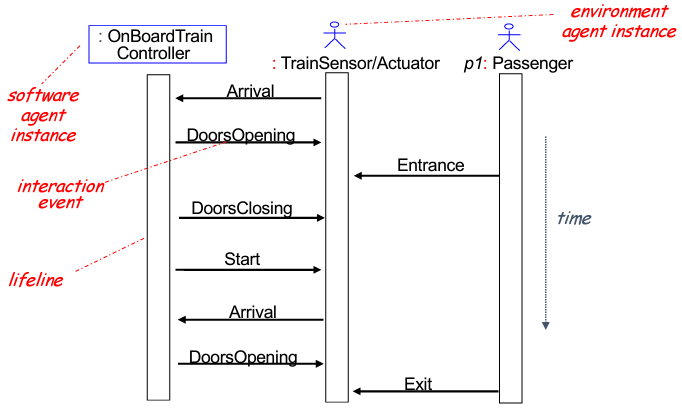
\includegraphics[scale=0.5]{img/sequence-diagram.png}
    \caption{Esempio di diagramma di sequenza \texttt{UML}}
\end{figure}
\begin{tcolorbox}[colback=orange!5!white,colframe=orange!75!black, title=Eventi]
    Gli eventi sono dei messaggi \textbf{istantanei} che vengono scambiati tra le varie
    istanze di agenti. Possono avere degli attributi che ne specificano il contenuto.
\end{tcolorbox}
Di fatto un evento corrisponde all'applicazione di un'operazione e sono tipicamente 
emessi da un'istanza di agente e ricevuti da una o più istanze di agente.

Nel sequence diagram abbiamo due tipologie di ordinamenti:
\begin{itemize}
    \item \textbf{Totale}: data una coppia di eventi possiamo dire quale evento è
    stato ricevuto prima dell'altro.
    \item \textbf{Parziale}: data una coppia di eventi non possiamo dire quale evento
    è stato ricevuto prima dell'altro.
\end{itemize}
\begin{figure}[H]
    \centering
    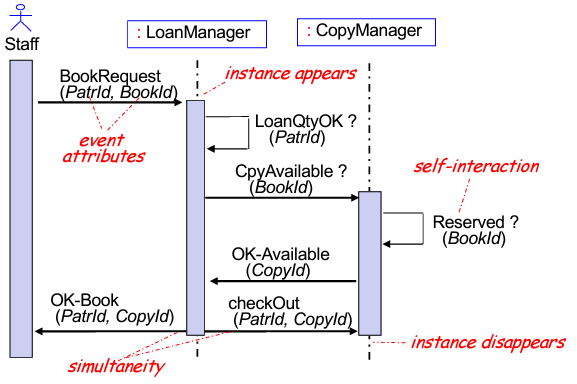
\includegraphics[scale=0.5]{img/sequence-ex.png}
    \caption{Esempio di diagramma di sequenza}
\end{figure}
\subsection{Raffinamento dei diagrammi di sequenza}
\subsubsection{Episodi}
Uno scenario che rappresentiamo potrebbe essere composto
da episodi, ovvero sotto-scenari.
\begin{figure}[H]
    \centering
    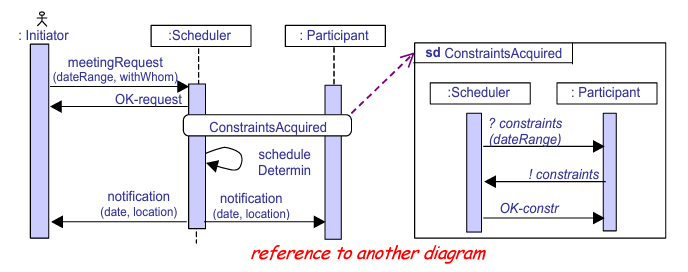
\includegraphics[scale=0.5]{img/sequence-episode.png}
\end{figure}

\subsubsection{Decomposizione degli agenti}
È possibile decomporre una responsabilità complicata su più agenti, in modo da
ridurre le granularità delle responsabilità.
\begin{figure}[H]
    \centering
    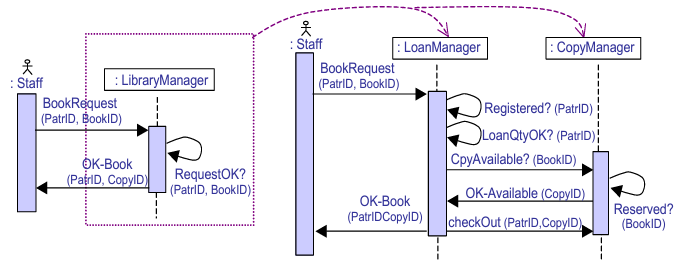
\includegraphics[scale=0.5]{img/agent-dec.png}
\end{figure}
\section{Modellare classi di comportamenti}
Una \textbf{macchina a stati} cerca di fornire tutti i possibili funzionamenti 
di un sistema, per farlo si utilizza una macchina a stati.

Un macchina a stati rappresenta una serie di transizioni tra stati
\[
S \times E \to S
\]
\begin{itemize}
    \item Gli stati sono finiti.
    \item Gli eventi sono finiti.
    \item Le state machine sono deterministiche.
\end{itemize}
\begin{figure}[H]
    \centering 
    \begin{tikzpicture}
        \umlbasicstate[x=0, y=0, name=state1, fill=gray!20]{Stato 1}
        \umlbasicstate[x=4, y=0, name=state2, fill=gray!20]{Stato 2}

        \umltrans[arg=evento1, pos=0.5]{state1}{state2}
    \end{tikzpicture}
\end{figure}
\subsubsection{Esempio pratico}
\begin{figure}[H]
    \centering
    \begin{tikzpicture}
        \begin{umlstate}[name=BookCopy, fill=blue!20]{BookCopyStatus}
            \umlstateinitial[name=state1, y=0.265]
            \umlbasicstate[x=3, y=0, name=state2, fill=gray!20]{Available}
            \umlbasicstate[x=9, y=0, name=state3, fill=gray!20]{OnLoan}
            \umlstatefinal[x=12, y=0.265, name=state4]

            \umltrans{state1}{state2}
            \umltrans[arg=checkOut, pos=0.5]{state2}{state3}
            \umlVHVtrans[arg=return, arm1=-2, pos=1.5]{state3}{state2}
            \umltrans[arg=lost, pos=0.5]{state3}{state4}
        \end{umlstate}
    \end{tikzpicture}
\end{figure}
Dal punto di vista semantico, una transizione ha luogo quando 
il sistema è in un particolare stato e occorre l'evento rappresentato.

Nei capitoli precedenti è stato definito il concetto di \textbf{stato} (\ref{sec:oggetto_concettuale}).

Quando parliamo delle state machine siamo più generici rispetto alla definizione precedente,
non ci riferiamo quindi a una particolare istanza di un oggetto, ma a una 
\textbf{classe di istanze oggetti}.
\subsection{Gli scenari come macchine a stati \texttt{UML}}
Tipicamente abbiamo una state machine per ogni variabile \textbf{controllata} da un agente.

Tipicamente le transizioni sono \textbf{istantanee}, mentre 
gli stati hanno una certa durata.
\begin{itemize}
    \item Possiamo rappresentare lo stato iniziale con un pallino pieno, che tipicamente 
    rappresenta l'istanziazione dello stato.
    \item Possiamo rappresentare lo stato finale con un pallino pieno con un cerchio attorno,
    che tipicamente rappresenta la terminazione dello stato.
\end{itemize}
Gli eventi possono avere degli attributi.
\begin{figure}[H]
    \centering
    \begin{tikzpicture}
        \begin{umlstate}[name=BookCopy, fill=blue!20]{BookCopyStatus}
            \umlstateinitial[name=state1, y=0.265]
            \umlbasicstate[x=3, y=0, name=state2, fill=gray!20]{Available}
            \umlbasicstate[x=9, y=0, name=state3, fill=gray!20]{OnLoan}
            \umlstatefinal[x=12, y=0.265, name=state4]

            \umltrans{state1}{state2}
            \umltrans[arg=checkOut(PatrId), pos=0.5]{state2}{state3}
            \umlVHVtrans[arg=return(PatrId), arm1=-2, pos=1.5]{state3}{state2}
            \umltrans[arg=lost, pos=0.5]{state3}{state4}
        \end{umlstate}
    \end{tikzpicture}
\end{figure}
Gli eventi si contraddistinguono in diverse varianti:
\begin{itemize}
    \item \textbf{Eventi esterni}: gli eventi esterni arrivano da un'altra state machine,
    che si suddividono in:
    \begin{itemize}
        \item \textbf{Eventi temporali}: all'arrivo di un certo orario succede qualcosa. 
        \item \textbf{Eventi di durata}: un evento che dura per un certo periodo di tempo.
        \item \textbf{Stimoli}: un evento che arriva dall'esterno, come per esempio da un
        agente. (\textit{Provenienti da un'altra state machine}).
    \end{itemize}
    \item \textbf{Eventi interni}: generati che è associato alla state machine.
    \textit{\textcolor{red}{DoorsClosing}} è un'applicazione dell'operazione
    \textcolor{red}{\textit{closeDoors}}.
\end{itemize}
\begin{tcolorbox}
    Usiamo il participio presente per gli eventi, mentre per le operazioni usiamo il
    verbo all'infinito.
\end{tcolorbox}
\subsubsection{Transizione automatiche}
Nel caso in cui non ci fosse alcuna etichetta che contraddistingue una transizione,
allora si tratta di una transizione automatica. Non sarà necessario che un evento
scateni la transizione.
\begin{figure}[H]
    \centering
    \begin{tikzpicture}
        \umlbasicstate[x=0, y=0, name=state1, fill=gray!20]{$S_1$}
        \umlbasicstate[x=4, y=0, name=state2, fill=gray!20]{$S_2$}
        \umltrans{state1}{state2}
    \end{tikzpicture}
\end{figure}
\subsubsection{Guardie per gli eventi}
Le guardie sono condizioni necessari per far si che un evento possa 
scatenare una transizione. Tipicamente si tratta di una condizione booleana.

È importante non confondere le condizioni necessarie con le condizioni 
sufficienti per far scattare una transizione.
La condizione necessarie è che la guardia sia vera, la condizione sufficiente
è che l'evento occorra.

Un esempio può essere \texttt{copyBorrowing[LatCopy]}.
\subsubsection{Azioni ausiliarie}
Le azioni ausiliarie sono condizioni che devono essere intraprese con una transizione 
va da uno stato ad un altro. Tipicamente si tratta di operazioni che vengono eseguite
un evento possa essere scatenato.

Un esempio può essere \texttt{DoorsOpening[AtPlatform and Speed = 0] /}
\texttt{Display}\\\texttt{terminalInfo}.
Tali operazioni sono atomiche e possono essere notifiche o azioni intraprese dall'ambiente 
quando la transizione avviene.
\subsubsection{Evitare transizioni inutili}

\begin{minipage}{0.45\textwidth}
    \begin{figure}[H]
        \centering
        \begin{tikzpicture}[scale=0.8, transform shape, every node/.style={font=\scriptsize}]
            \umlstateinitial[name=ini, x= -2, y=0.265]
            \umlbasicstate[x=0, y=0, name=state1, fill=gray!20]{Iddle}
            \umlbasicstate[x=5, y=0, name=state2, fill=gray!20]{CardInserted}
            \umlbasicstate[x=0, y=-4, name=state3, fill=gray!20]{CardRead}
            \umlbasicstate[x=5, y=-4, name=state4, fill=gray!20]{CardValidated}
    
            \umltrans{ini}{state1}
            \umltrans[arg=CardInsertion, pos=0.5]{state1}{state2}
            \umltrans{state2}{state3}
            \umltrans{state3}{state4}
            
        \end{tikzpicture}
    \end{figure}
\end{minipage}
\begin{minipage}{0.50\textwidth}
    \begin{figure}[H]
        \centering
        \begin{tikzpicture}[scale=0.8, transform shape, every node/.style={font=\scriptsize}]
            \umlstateinitial[name=ini, x= -2, y=0.265]
            \umlbasicstate[x=0, y=0, name=state1, fill=gray!20]{Iddle}
            \umlbasicstate[x=5, y=0, name=state2, fill=gray!20]{CardInserted}
            \umlbasicstate[x=5, y=-4, name=state3, fill=gray!20]{CardValidated}
    
            \umltrans{ini}{state1}
            \umltrans[arg=CardInsertion, pos=0.5]{state1}{state2}
            \umltrans[arg={/readCard}, pos=0.5]{state2}{state3}
            
        \end{tikzpicture}
    \end{figure}
\end{minipage}

Invece di rappresentare uno stato intermedio utilizzo un'azione ausiliaria per
rappresentare la lettura della carta.
\subsubsection{Notifica degli eventi}
Nel contesto del goal model potrebbe aver senso il meccanismo delle notifiche, in quanto 
potremmo avere una relazione tra due state machine distinte, avendo che alcuni eventi 
possono essere notificati da una state machine all'altra.

Ad esempio \texttt{send BookInfo.copyReturn}. Dove BooInfo è la state machine che
riceverà l'evento, mentre copyReturn è l'evento che verrà notificato.
\subsubsection{Azioni di entrata e uscita}
Gli eventi di entrata e uscita etichettano eventi che avvengono quando si entra o si esce
da un particolare stato. Permettendoci di evitare duplicati.

Invece di etichettare tutti gli stati di ingresso etichettiamo lo stato con 
\texttt{entry/ <azione>}, mentre per gli stati di uscita etichettiamo lo stato con
\texttt{exit/ <azione>} per evitare di duplicare le etichette in uscita.
\subsection{Raffinamento delle macchine a stati}
\subsubsection{Decomposizione sequeziale degli stati}
È possibile rappresentare una state machine all'interno di un'altra state machine,
esplodendo lo stato in una serie di sotto-stati. Allo stesso modo possiamo rappresentare 
le due state machine in due diagrammi separati. rappresentando la relazione tra le due
state machine.
\subsubsection{Decomposizione parallela}
È possibile rappresentare due state machine in parallelo, in modo da rappresentare
come lo stato del sistema evolva in parallelo a seconda di due proprietà distinte.

La rappresentazione d'esempio piò essere la transizione da treno fermo a treno in movimento 
e parallelamente da porte chiuse a porte aperte, che avvengono in parallelo.

\subsubsection{Fork e join}
Dopo aver rappresentato due state machine in parallelo, possiamo rappresentare
il punto in cui le due state machine si incontrano, ovvero il punto in cui
le due state machine si riuniscono. Allo stesso modo possiamo rappresentare
il punto in cui le due state machine si dividono.

Per farlo utilizziamo i nodi di \texttt{fork} e \texttt{join}.
\section{Costruire modelli di comportamento}
\subsection{Goal, scenari e state machine sono complementari}
\subsubsection{Goal model}
\begin{tcolorbox}[colback=green!5!white,colframe=green!75!black, title=Vantaggi del goal model]
    \begin{itemize}
        \item Hanno una rappresentazione dichiarativa, aiutano quindi a capire
        \textit{quando} e da \textit{chi} viene soddisfatto un goal.
        \item Rappresentazione di aspetti funzionali e non funzionali.
        \item Rappresentano tanti funzionamenti.
        \item Può essere usato in analisi preliminari.
    \end{itemize}
\end{tcolorbox}
\begin{tcolorbox}[colback=red!5!white,colframe=red!75!black, title=Limiti del goal model]
    \begin{itemize}
        \item Molte cose rimangono implicite, non spiego \textit{come} il goal viene
        soddisfatto.
        \item Troppo astratto.
        \item Difficile da elicitare.
    \end{itemize}
\end{tcolorbox}
\subsubsection{Scenari}
\begin{tcolorbox}[colback=green!5!white,colframe=green!75!black, title=Vantaggi degli scenari]
    \begin{itemize}
        \item Esempi concreti e narrativi.
        \item Facili da elicitare.
        \item Rappresentano comportamenti espliciti.
        \item Utili per i test di accettazione.
    \end{itemize}
\end{tcolorbox}
\begin{tcolorbox}[colback=red!5!white,colframe=red!75!black, title=Limiti degli scenari]
    \begin{itemize}
        \item La copertura completa è difficile, ogni sequence diagram rappresenta
        una sola esecuzione.
        \item Ragionare in termini potrebbe introdurre dei bias, rappresentando 
        come il sistema funzionerà, con scelte premature (\textit{potrebbero introdurre 
        scelte architetturali premature}).
    \end{itemize}
\end{tcolorbox}
\subsubsection{State machine}
\begin{tcolorbox}[colback=green!5!white,colframe=green!75!black, title=Vantaggi delle state machine]
    \begin{itemize}
        \item Rappresentazione visuale.
        \item Rappresentazione esplicita di comportamenti del sistema (\textit{classi}).
        \item Verificabile e eseguibile.
        \item Supporta la generazione di codice.
    \end{itemize}
\end{tcolorbox}
\begin{tcolorbox}[colback=red!5!white,colframe=red!75!black, title=Limiti delle state machine]
    \begin{itemize}
        \item Requisiti impliciti, quindi troppo operazionale.
        \item Difficile da costruire e da capire.
    \end{itemize}
\end{tcolorbox}